% !TEX encoding = UTF-8
% !TEX TS-program = pdflatex
% !TEX root = ../tesi.tex
% !TEX spellcheck = it-IT

%**************************************************************
\chapter{Conclusioni}
\label{cap:conclusioni}
%**************************************************************

In questo capitolo finale vengono tratte le conclusioni riguardo alle attività svolte durante il periodo di stage.

\section{Valutazione del risultato e di React Native}

\begin{figure}[htp]
\centering
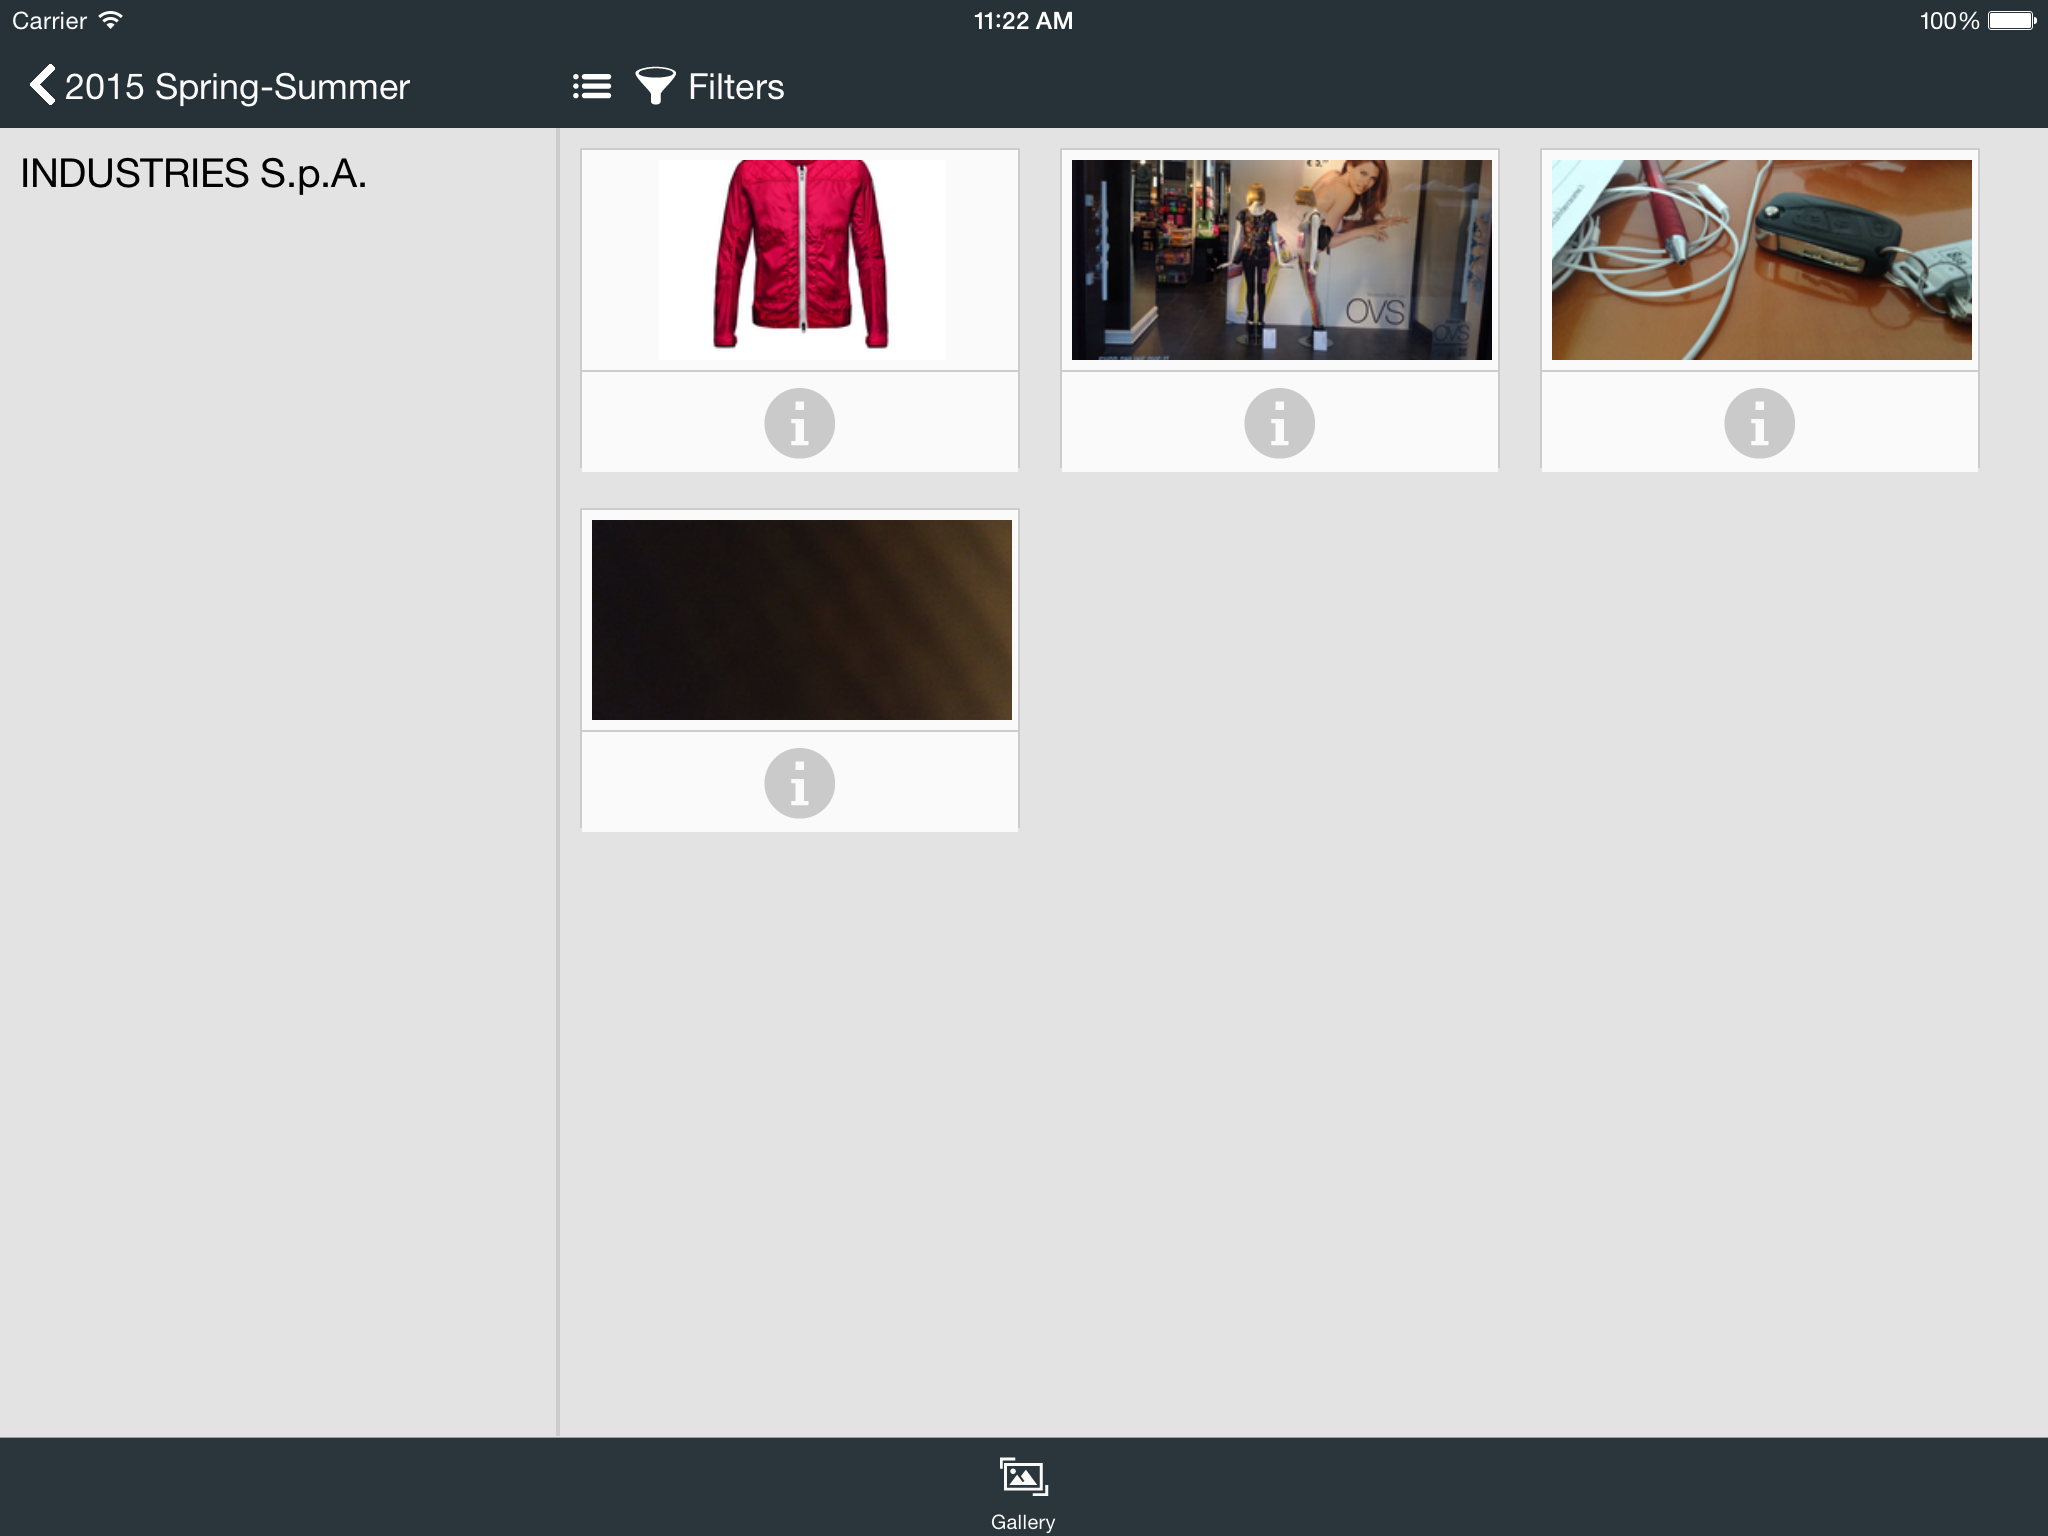
\includegraphics[width=\textwidth]{../immagini/wg-gallery}
\caption{Screenshot dell'applicazione realizzata}  
\end{figure}

L'applicazione sviluppata soddisfa in pieno le aspettative dell'azienda, in quanto risulta più fluida rispetto all'applicazione attuale, dimostrando che l'utilizzo di un framework diverso da quello utilizzato fino ad oggi dall'azienda permette di ottenere prestazioni migliori.

Considerando inoltre che l'applicazione sviluppata non utilizza particolari ottimizzazioni si ritiene che ci sia un ulteriore margine di miglioramento.

Questo è stato reso possibile da React Native, il quale ha permesso di sviluppare un'applicazione nativa come se fosse una normale applicazione web, garantendo una velocità di apprendimento notevole.

React Native non è ancora perfetto, infatti, durante lo sviluppo dell'applicazione si sono riscontrati alcuni bug all'interno del framework, dovuti principalmente al fatto che si tratta di un framework ancora giovane.
In ogni caso, la maggior parte di questi bug sono stati, di volta in volta, risolti dalle release avvenute durante il periodo di sviluppo dell'applicazione, segno che gli sviluppatori di React Native sono attenti ai problemi segnalati dalla community.

Considerando anche il workflow di sviluppo che offre il framework e il tool di supporto presenti, la valutazione di React Native non può essere altro che positiva.

Inoltre, la roadmap di React Native prevede la pubblicazione della versione per Android e ulteriori ottimizzazioni e funzionalità, il tutto supportato da Facebook che sta attualmente utilizzando React Native per alcune delle sue applicazioni pubblicate nell'App Store di iOS e nel Google Play Store.

%\todo[inline]{eventualmente aggiungere la storia della continuos delivery, magari fare un'appendice}

\subsection{Requisiti soddisfatti}

L'applicazione soddisfa tutti i requisiti obbligatori e desiderabili individuati, mentre dei requisiti facoltativi non viene soddisfatto il requisito
\textbf{RFF2.2.2} - \textit{L'utente deve poter effettuare il pinch-to-zoom sull'immagine}.

In totale sono stati soddisfatti 47 su 48 requisiti funzionali, mentre sono stati soddisfatti tutti e 4 i requisiti di vincolo.
%\todo{Aggiornare questa frase se si implementa la pagina di login}

Per misurare la fluidità dell'applicazione è stato utilizzato il FPS Monitor offerto da React Native, il quale ha rilevato una media di 60 FPS durante l'utilizzo dell'applicazione.

Durante il caricamento di ulteriori dati nella visualizzazione a griglia si è registrato la maggior parte delle volte un leggero calo degli FPS che da 60 scendono a 54-55.
Solo una volta l'applicazione è scesa a 34 FPS per un breve periodo di tempo.

Considerando che il minimo numero di FPS necessari perché un'interfaccia grafica risulti fluida all'occhio umano è di 30 FPS, il risultato ottenuto è più che accettabile.

\section{Aspetti critici e possibili estensioni}

Gli unici problemi incontrati con l'utilizzo di React Native riguardano alcuni bug, ma come è già stato detto, questi sono dovuti al fatto che si tratta di un framework nuovo ed in ogni caso, i bug segnalati il più delle volte vengono risolti dalla release successiva.

Per quanto riguarda l'applicazione, l'aspetto grafico è stato lasciato in secondo piano e quindi può essere migliorato, specialmente per quanto riguarda l'aspetto dei pulsanti e delle icone.

Questa scelta è stata fatta dal momento che lo scopo principale dell'applicazione è quello di valutare se l'utilizzo di un framework diverso possa portare alla realizzazione di un'applicazione migliore rispetto al client per iPad attuale.

L'applicazione sviluppata è quindi considerata dall'azienda come un prototipo e conseguentemente non è prevista una futura manutenzione del codice. 

Si è scelto di non implementare i test d'unità con Jest e di non utilizzare Flow per l'analisi statica, in quanto è stato ritenuto più interessante provare ad implementare funzionalità aggiuntive offerte dal framework come le animazioni, piuttosto che concentrarsi sulla qualità del codice.

%Per lo stesso motivo non sono stati sviluppati test d'unità con Jest in quanto è stato ritenuto più interessante provare ad implementare funzionalità aggiuntive offerte dal framework come le animazioni, piuttosto che implementare dei test.

Sempre riguardo l'applicazione sviluppata, è stata implementa solamente la visualizzazione della gallery, trascurando tutte le altre funzionalità offerte dal client attuale, come ad esempio la pagina di autenticazione, la creazione di nuovi assets e la possibilità di utilizzare la parte collaborativa del sistema WARDA.

Tali funzionalità non sono state analizzate e implementate per motivi di tempo.

\section{Conoscenze acquisite}

Durante le attività di stage sono state acquisite competenze sia nello sviluppo di applicazioni mobile, sia in altri settori ad esso correlati.

Principalmente è stato studiato come è possibile sviluppare applicazioni mobile utilizzando JavaScript, sia sotto forma di applicazioni ibride che come applicazioni native, analizzando le varie strategie utilizzate per astrarre le API native dei dispositivi mobile.

Inoltre, i framework analizzati durate il periodo di stage erano totalmente sconosciuti, mentre al termine dello stage sono state acquisite delle conoscenze basilari riguardo i vari framework.
In particolar modo per quanto riguarda React Native è stata raggiunta una buona padronanza del framework, specialmente nello sviluppo di un'applicazione secondo i pattern tipici, anch'essi sconosciuti prima dell'inizio dello stage.

Sempre legato allo sviluppo, si sono acquisite delle competenze riguardo ai tools offerti da Xcode per il debug di applicazioni native, che prima non erano mai stati utilizzati.

Sono state inoltre rafforzate le competenze riguardo il linguaggio JavaScript, che era già noto prima dello stage, ma del quale non ero a conoscenza dello standard ES6 e la sintassi JSX.

In secondo luogo sono state acquisite delle nozioni riguardo alcuni aspetti del mondo aziendale, in particolare si è potuto osservare come un'azienda valuta le caratteristiche di un framework per stimare i benefici e i costi derivanti dall'introduzione di tale framework nel processo di sviluppo.

Inoltre è stato possibile osservare come l'esperienza utente e i feedback forniti dai clienti influiscano sulla progettazione di un'interfaccia grafica e portino ad adottare determinate strategie per massimizzare le prestazioni al fine di soddisfare le loro esigenze.

Infine, utilizzando le API REST di WARDA è stato possibile osservare come viene utilizzata l'architettura REST a livello aziendale e come creare un'applicazione che utilizzi tali API.
